\chapter{bayesreg objects}
\label{bayesreg} \index{bayesreg object}

{\em Authors: Andreas Brezger, Stefan Lang and Thomas Kneib} \\
{\em email:
\href{mailto:andib@stat.uni-muenchen.de}{andib@stat.uni-muenchen.de},
\href{mailto:lang@stat.uni-muenchen.de}{lang@stat.uni-muenchen.de}}
and
{\em\href{mailto:kneib@stat.uni-muenchen.de}{kneib@stat.uni-muenchen.de}} \\
\vspace{0.3cm}


{\em bayesreg objects} are used to fit (multivariate) generalized
linear models or hazard rate models with a {\em Structured Additive
Predictor (STAR)}, see Fahrmeir, Kneib, and Lang (2004). Inference
is fully Bayesian via Markov Chain Monte Carlo (MCMC) techniques.
The methodological background is provided in considerable detail in
the methodology manual. More details can be found in Fahrmeir and
Lang (2001a), Fahrmeir and Lang (2001b), Lang and Brezger (2004),
Brezger and Lang (2005), Fahrmeir and Osuna (2003), Hennerfeind,
Brezger and Fahrmeir (2005), and Fahrmeir and Hennerfeind (2003).
Good introductions into generalized linear models are the monographs
of Fahrmeir and Tutz (2001) and Mc Cullagh and Nelder (1989).
Introductions to semi- and nonparametric models are given in Green
and Silverman (1994), Hastie and Tibshirani (1990), Hastie and
Tibshirani (1993) and Hastie, Tibshirani and Friedman (2001). The
paper of Chib and Greenberg (1995), the monograph {\em Markov Chain
Monte Carlo in Practice} edited by Gilks, Richardson and
Spiegelhalter (1996) and the article by Green (2001) give a good
overview over MCMC simulation techniques.

First steps with {\em bayesreg objects} can be done with the
tutorial like example in chapter \ref*{zambiaanalysis} of the
tutorials manual.

\clearpage

\section{Method regress}
\label{bayesregress} \index{bayesreg object!regress command}

\subsection{Description}
\label{bayesregregressdescr}

Method #regress# estimates regression or hazard rate models with
Structured Additive Predictor. An introduction to the methodological
background can be found in the methodology manual.

\index{generalized linear models} \index{generalized additive
models} \index{varying coefficients models} \index{Bayesian
semiparametric regression} \index{MCMC} \index{Markov chain Monte
Carlo}



\subsection{Syntax}
\label{bayesregregresssyntax}

 #>#{\em objectname}.#regress# {\em model} [#weight# {\em weightvar}] [#if# {\em expression}] [{\em , options}] #using# {\em dataset}

Method #regress# estimates the regression model specified in {\em
model} using the data specified in {\em dataset}. {\em dataset}
must be the name of a {\em dataset object} created before. The
details of correct models are covered in \autoref{modelsyntax}.
The distribution of the response variable can be either Gaussian,
gamma, binomial, multinomial, Poisson, negative binomial,
zero inflated Poisson or zero inflated negative binomial, see
also \autoref{familyopt} for an overview about the distributions
supported by {\em BayesX}. The response distribution is specified
using option #family#, see \autoref{familysyntax} below and the
options list in \autoref{regressoptions} for a detailed
description. The default is #family=binomial# with a logit link.
An #if# statement may be specified to analyze only a part of the
data set, i.e.~the observations where {\em expression} is true.

\subsubsection{Optional weight variable }
\label{weightspecification}

An optional weight variable {\em weightvar} may be specified to
estimate weighted regression models. For Gaussian responses {\em
BayesX} assumes that $y_r|\eta_r,\sigma^2 \sim
N(\eta,\sigma^2/weightvar_r)$. Thus, for grouped Gaussian
responses the weights must be the number of observations in the
groups if the $y_r$'s are the average of individual responses. If
the $y_r$'s are the sum of responses in every group, the weights
must be the reciprocal of the number of observations in the
groups. Of course, estimation of usual weighted regression models
with heteroscedastic errors  is also possible. In this case the
weights should be proportional to the reciprocal of the
heteroscedastic variances. If the response distribution is
binomial, it is assumed that the values of the weight variable
correspond to the number of replications and that the values of
the response variable correspond to the number of successes. If
#weight# is omitted, {\em BayesX} assumes that the number of
replications is one, i.e.~the values of the response must be
either zero or one. For grouped Poisson data the weights must be
the number of observations in a group and the $y_i$'s are assumed
to be the average of individual responses. In the case of gamma
distributed responses {\em BayesX} assumes $y_r \sim
G(\exp(\eta_r),\nu/weightvar_r)$ where $\mu_r= \exp(\eta_r)$ is
the mean and $s_r = \nu/weightvar_r$ is the scale parameter.

If estimation is based on latent utility representations, the
specification of weights is not allowed. Also for negative
binomial, zero inflated Poisson and zero inflated negative
binomial models is weighted regression not implemented.

\subsubsection{Syntax of possible model terms}
\label{modelsyntax}

The general syntax of models is:

$depvar = term_1 + term_2 + \cdots + term_r$

{\em depvar} specifies the dependent variable in the model and
$term_1$,\dots,$term_r$ define in which way the covariates
influence the dependent variable. The different terms must be
separated by '+' signs. A constant intercept is automatically
included in the models and must not be specified by the user. This
section reviews all possible model terms that are supported in the
current version of {\em bayesreg objects} and provides some
specific examples. Note that all described terms may be combined
in arbitrary order. An overview about the capabilities of {\em
bayesreg objects} is given in \autoref{terms}.
\autoref{bayesreginteractions} shows how interactions between
covariates are specified. Full details about all available options
are given in \autoref{localoptions}.

Throughout this section #Y# denotes the dependent variable.

\subsubsection*{Offset}

\begin{itemize}
\item[] {\em Description}: Adds an offset term to the predictor.
\item[] {\em Predictor}: $\eta =  \cdots + \mbox{\it offs} + \cdots$
\item[] {\em Syntax}: #offs(offset)#
\item[] {\em Example}:

For example, the following model statement can be used to estimate
a Poisson model with #offs# as offset term and #W1# and #W2# as
fixed effects (if #family=poisson# is specified in addition):

\texttt{Y = offs(offset) + W1 + W2}

\end{itemize}

\subsubsection*{Fixed effects}

\begin{itemize}
\item[] {\em Description}: Incorporates covariate #W1# as a fixed effect into the model.
\item[] {\em Predictor}: $\eta =  \cdots + \gamma_1 W1 + \cdots$
\item[] {\em Syntax}: #W1#
\item[] {\em Example}:

The following model statement causes {\em BayesX} to estimate a
model with $q$ fixed (linear) effects:

\texttt{Y = W1 + W2 + $\cdots$ + Wq}
\end{itemize}

\subsubsection*{Nonlinear effects of continuous covariates and time
scales}

\begin{itemize}
 \item[]{\bf\sffamily First or second order random walk}
 \item[]{\em Description}: Defines a first or second order random walk
 prior for the effect of #X1#.
 \item[]{\em Predictor}: $\eta = \cdots + f_1(X1) + \cdots $
 \item[] {\em Syntax}:

#X1(rw1#[, {\em options}]#) #

#X1(rw2#[, {\em options}]#) #
\item[] {\em Example}:

Suppose we have a continuous covariate #X1#, whose effect is
assumed to be nonlinear. The following model statement defines a
second order random walk prior for $f_1$:

#Y = X1(rw2,a=0.001,b=0.001)#

Here, the expression #X1(rw2,a=0.001,b=0.001)# indicates, that the
effect of #X1# should be incorporated nonparametrically into the
model using a second order random walk prior. A first order random
walk is specified in the model statement by modifying the first
argument in #X1(rw2,a=0.001,b=0.001)# from #rw2# to #rw1# which
yields the term #X1(rw1,a=0.001,b=0.001)#. The second and third
argument in the expression above are used to specify the
hyperparameters of the inverse gamma prior for the variance.
Besides the options #a# and #b# some more options are available,
see \autoref{localoptions} for details.

\item[] {\bf\sffamily P-spline with first or second order random
walk penalty}

\item[] {\em Description}: Defines a P-spline with a first or
second order random walk penalty for the parameters of the spline.
\item[] {\em Predictor}: $\eta =  \cdots + f_1(X1) + \cdots$
\item[] {\em Syntax}:

#X1(psplinerw1#[{\em , options}]#) #

#X1(psplinerw2#[{\em , options}]#) #
\item[] {\em Example}:

For example, a P-spline with second order random walk penalty is
obtained using the following model statement:

#Y = X1(psplinerw2)#

By default, the degree of the spline is 3 and the number of inner
knots is 20. The following model term defines a quadratic P-spline
with 30 knots:

#Y = X1(psplinerw2,degree=2,nrknots=30)#

Full details about all possible options for P-splines are given in
\autoref{localoptions}.

\item[] {\bf\sffamily Seasonal component for time scales}

\item[] {\em Description}: Defines a seasonal effect of #time#.
\item[] {\em Predictor}: $\eta =  \cdots + f_{season}(time) +
\cdots $ \item[] {\em Syntax}:

#time(season#[, {\em options}]#) #
\item[] {\em Example}:

A seasonal component for a time scale #time# is specified for
example by

#Y = time(season,period=12)#.

Here, the second argument specifies the period of the seasonal
effect. In the example above the period is 12, corresponding to
monthly data.
\end{itemize}


\subsubsection*{Spatial Covariates}

\begin{itemize}
\item[]{\bf\sffamily Markov random field}

\item[] {\em Description}:

Defines a Markov random field prior for the spatial covariate
#region#. {\em BayesX} allows an appropriate incorporation of
spatial covariates with geographical information stored in the {\em
map object} specified through the option #map#.
\item[] {\em Predictor}: $\eta = \cdots + f_{spat}(region) + \cdots$
\item[] {\em Syntax}:

#region(spatial,map=#{\em characterstring}#[#{\em , options}]#) #
\item[] {\em Example}:

The specification of a Markov random field prior for spatial data
has #map# as a required argument which must be the name of a {\em
map object} (see \autoref{map}) that contains all necessary
spatial information about the geographical map, i.e.~the neighbors
of each region and the weights associated with the neighbors. For
example the statement

#Y = region(spatial,map=germany)#

defines a Markov random field prior for #region# where the
geographical information is stored in the {\em map object}
#germany#. An error will be raised if #germany# is not existing.
It is advisable to reorder the regions of a map in advance to
obtain a band matrix like precision matrix. This is achieved using
method #reorder# of {\em map objects}, see \autoref{mapreorder}
for details.

\item[]{\bf\sffamily 2 dimensional P-spline with first order
random walk penalty}

\item[] {\em Description}:

Defines a 2 dimensional P-spline for the spatial covariate
#region# based on the tensor product of 1 dimensional P-splines
with a 2 dimensional first order random walk penalty for the
parameters of the spline. Estimation is based on the coordinates
of the centroids of the regions an observation pertains to. The
centroids are computed using the geographical information stored
in the {\em map object} specified through the option #map#.
\item[] {\em Predictor}: $\eta= \cdots + f(centroids) + \cdots$
\item[] {\em Syntax}:

#region(geospline,map=#{\em characterstring}#[, #{\em options}]#) #
\item[] {\em Example}:

The specification of a 2 dimensional P-spline ({\em geospline})
for spatial data has #map# as a required argument which must be
the name of a {\em map object} (see \autoref{map}) that contains
all necessary spatial information about the geographical map,
i.e.~the neighbors of each region and the weights associated with
the neighbors. The model term

#Y = region(geospline,map=germany)#

specifies a tensor product cubic P-spline with first order random
walk penalty where the geographical information is stored in the
{\em map object} #germany#.
\end{itemize}

\subsubsection*{Unordered group indicators}

\begin{itemize}
\item[]{\bf\sffamily Unit- or cluster-specific unstructured
effect}

\item[] {\em Description}: Defines an unstructured (uncorrelated)
random effect with respect to grouping variable #grvar#. \item[]
{\em Predictor}: $\eta = \cdots + f(grvar) + \cdots$ \item[] {\em
Syntax}:

#grvar(random#[, {\em options}]#) #
\item[] {\em Example}:

{\em BayesX} also supports Gaussian i.i.d.~random effects to cope
with unobserved heterogeneity among units or clusters of
observations. Suppose the analyzed data set contains a group
indicator #grvar# that gives information about the individual or
cluster a particular observation belongs to. Then an individual
specific uncorrelated random effect is incorporated through the
term

#Y = grvar(random)#

The inclusion of more than one random effects term in the model is
possible allowing the estimation of multilevel models. However, we
have only limited experience with multilevel models so that it is
not clear how well these models can be estimated in {\em BayesX}.
\end{itemize}

\subsubsection*{Nonlinear baseline effect in Cox models}

\begin{itemize}
\item[]{\bf\sffamily P-spline with second order random walk
penalty}

\item[] {\em Description}: Defines a P-spline with a second order
random walk penalty for the parameters of the spline for the
log-baseline effect $\log(\lambda_0$(#time#)). \item[] {\em
Predictor}: $\eta = \log(\lambda_0(time)) + \cdots$ \item[] {\em
Syntax}:

#time(baseline#[, {\em options}]#) #
\item[] {\em Example}:

Suppose continuous-time survival data (#time#, #delta#) together
with additional covariates (#W1#,#X1#) are given where #time#
denotes the vector of observed duration times, #delta# is the
vector of corresponding indicators of non-censoring, #W1# is a
discrete covariate and #X1# a continuous one. The following Cox
model with hazard rate $\lambda$ and log-baseline effect
$\log(\lambda_0$(#time#))
\[
\lambda(time)=\lambda_0(time)\exp (\gamma_0 + \gamma_1 W1 + f(X1)
)=\exp\left(\log(\lambda_0(time)) + \gamma_0 + \gamma_1 W1 +
f(X1)\right)
\]
is estimated by the model statement

#delta = time(baseline) + W1 + X1(psplinerw2)#

Note that a baseline term has to be specified in the model.
\end{itemize}

\subsubsection*{Varying coefficients with continuous covariates as
effect modifier}
\medskip

\begin{itemize}
\item[]{\bf\sffamily First or second order random walk}

\item[] {\em Description}:

Defines a varying coefficient term, where the effect of #X1#
varies smoothly over the range of #X2#. Covariate #X2# is the
effect modifier. The smoothness prior for $f$ is a first or second
order random walk.
\item[] {\em Predictor}: $\eta= \cdots + f(X2)X1 + \cdots$
\item[] {\em Syntax}:

#X1*X2(rw1#[, {\em options}]#) #

#X1*X2(rw2#[, {\em options}]#) #
\item[] {\em Example}:

For example, a varying coefficient term with a second order random
walk smoothness prior is defined as follows:

#Y = X1*X2(rw2)#

\item[] {\bf\sffamily P-spline with first or second order random
walk penalty}

\item[] {\em Description}:

Defines a varying coefficient term, where the effect of #X1#
varies smoothly over the range of #X2#. Covariate #X2# is the
effect modifier. The smoothness prior for $f$ is a P-spline with
first or second order random walk penalty.
\item[] {\em Predictor}: $\eta= \cdots + f(X2)X1 + \cdots$
\item[] {\em Syntax}:

#X1*X2(psplinerw1#[, {\em options}]#) #

#X1*X2(psplinerw2#[, {\em options}]#) #
\item[] {\em Example}:

For example, a varying coefficient term with a second order random
walk smoothness prior is defined as follows:

#Y = X1*X2(psplinerw2)#

\item[]{\bf\sffamily Seasonal prior}

\item[] {\em Description}:

Defines a varying coefficients term where the effect of #X1# varies
over the range of the effect modifier #time#. For #time# a seasonal
prior is used.
\item[] {\em Predictor}: $\eta= \cdots + f_{season}(time)X1 + \cdots $
\item[] {\em Syntax}:

#X1*time(season#[, {\em options}]#) #
\item[] {\em Example}:

The inclusion of a varying coefficients term with a seasonal prior
may be meaningful if we expect a different seasonal effect with
respect to grouping variable #X1#. In this case we can include
additional seasonal effects for each category of #X1# by

#Y = X1*time(season) #

\end{itemize}

\subsubsection*{Time-varying effects in Cox models}

\begin{itemize}
\item[]{\bf\sffamily P-spline with second order random walk
penalty}

\item[] {\em Description}: Defines a varying coefficients term
where the effect of #X1# varies over the range of the effect
modifier #time#, i.e. variable #X1# has time-varying effect. The
smoothness prior for $f($#time#$)$ is a P-spline with second order
random walk penalty.

 \item[] {\em Predictor}: $\eta = \log(\lambda_0(time)) +
f(time)X1 \cdots$ \item[] {\em Syntax}:

 #X1*time(baseline#[, {\em options}]#) #
 \item[] {\em Example}:

Suppose continuous-time survival data (#time#, #delta#) together
with an additional covariate #X1# are given, where #time# denotes
the vector of observed duration times, #delta# is the vector of
corresponding indicators of non-censoring. The following Cox model
with hazard rate $\lambda$
\begin{eqnarray*}
 \lambda(time) & = & \lambda_0(time)\exp(\gamma_0 + f(time)X1)\\
 & = & \exp\left(\log(\lambda_0(time)) + \gamma_0 + f(time)X1\right)
\end{eqnarray*}
is estimated by the model statement

#delta = time(baseline) + X1*time(baseline)#

\end{itemize}


\subsubsection*{Varying coefficients with spatial covariates as
effect modifiers}

\begin{itemize}
\item[]{\bf\sffamily Markov random field}

\item[] {\em Description}:

Defines a varying coefficient term where the effect of #X1# varies
smoothly over the range of the spatial covariate #region#. A
Markov random field is estimated for $f_{spat}$. The geographical
information is stored in the {\em map object} specified through
the option #map#.
\item[] {\em Predictor}: $\eta = \cdots + f_{spat}(region)X1 + \cdots$
\item[] {\em Syntax}:

#X1*region(spatial,map=#{\em characterstring}#[,#{\em options}]#) #
\item[] {\em Example}:

For example the statement

#Y = X1*region(spatial,map=germany) #

defines a varying coefficient term with the spatial covariate
#region# as the effect modifier and a Markov random field as spatial
smoothness prior. Weighted Markov random fields can be estimated by
including an appropriate weight definition when creating the {\em
map object} #germany# (see \autoref{mapinfile}).
\end{itemize}


%{\em 2 dimensional P-spline with first order random walk penalty}
%\begin{itemize}
%\item[] {\em Description}:

%Defines a varying coefficients term where the effect of X1 varies
%smoothly over the range of the spatial covariate X2. A 2
%dimensional P-spline based on the tensor product of 1 dimensional
%P-splines with a 2 dimensional first order random walk penalty for
%the parameters of the spline is estimated for $f$. The centroids
%are computed using the geographical information stored in the map
%object specified through the option #map#.
%\item[] {\em Predictor}: $\eta= \cdots + f(centroids)X1 + \cdots$
%\item[] {\em Syntax}:

%X1*X2(geospline,map=characterstring[, options])
%\item[] {\em Example}:
%\end{itemize}


\subsubsection*{Varying coefficients with unordered group indicators as effect modifiers
(random slopes)}

\begin{itemize}
\item[]{\bf\sffamily Unit- or cluster-specific unstructured
effect}

\item[] {\em Description}:

Defines a varying coefficient term where the effect of #X1# varies
over the range of the group indicator #grvar#. Models of this type
are usually referred to as random slope models. A  Gaussian
i.i.d.~random effect with respect to grouping variable #grvar# is
assumed for $f$. A main effect $\gamma X1$ is additionally
estimated using a diffuse prior for $\gamma$. This means that the
random slope effect $f(grvar)X1$ can be seen as the deviation from
the main effect. Estimation is carried out using hierarchical
centering, see Gelfand, Sahu and Carlin (1995). Note that
nonsensical results are obtained if an additional fixed effect of
#X1# is added in the model statement because the fixed effect is
automatically estimated.
\item[] {\em Predictor}: $\eta = \cdots + \gamma X1 + f(grvar)X1 + \cdots$
\item[] {\em Syntax}:

#X1*grvar(random#[, {\em options}]#) #
\item[] {\em Example}:

For example, a random slope term with incorporation of #X1# as
fixed effect is specified as follows:

#Y = X1*grvar(random)#

If the linear effect of #X1# should be omitted, the option
#nofixed# must be specified:

#Y = X1*grvar(random,nofixed)#
\end{itemize}


\subsubsection*{Surface estimators}

\begin{itemize}
\item[] {\bf\sffamily 2 dimensional P-spline with first order
random walk penalty}

\item[] {\em Description}:

Defines a 2 dimensional P-spline based on the tensor product of 1
dimensional P-splines with a 2 dimensional first order random walk
penalty for the parameters of the spline.
\item[] {\em Predictor}: $\eta= \cdots + f(X1,X2) + \cdots$
\item[] {\em Syntax}:

#X1*X2(pspline2dimrw1#[, {\em options}]#) #
\item[] {\em Example}:

The model term

#Y = X1*X2(pspline2dimrw1)#

specifies a tensor product cubic P-spline with first order random
walk penalty.

In many applications it is favorable to additionally incorporate
the 1 dimensional main effects of #X1# and #X2# into the models.
In this case the 2 dimensional surface can be seen as the
deviation from the main effects. Note, that the number of inner
knots has to be the same for the main effects and the interaction
effect. For example, splines with 10 inner knots are estimated by


 #Y = X1(psplinerw2,nrknots=10) + X2(psplinerw2,nrknots=10)#\\
 #    + X1*X2(pspline2dimrw1,nrknots=10)#
\end{itemize}



\subsubsection{Description of additional options for terms of bayesreg objects}
\label{localoptions}

All arguments described in this section are optional and may be
omitted. Generally, options are specified by adding the option
name to the specification of the model term type in the
parentheses, separated by comma. Boolean options are specified by
simply adding the option name to the options of a certain term.
For example, a random intercept term with #a=b=0.001# as
parameters for the inverse gamma distribution of the variance
parameter, with updating according to IWLS and without
incorporation of #X1# as fixed effect is specified as follows:

#X1*grvar(random,a=0.001,b=0.001,proposal=iwls,nofixed)#

Note that all options may be specified in arbitrary order.
\autoref{options} provides explanations and the default values of
all possible options. In \autoref{termsoptions} all reasonable
combinations of model terms and options can be found.



%------------------------------------------------------------------------------%

\begin{table}[ht] \footnotesize
\begin{center}
\begin{tabular}{|p{2.8cm}|p{3.6cm}|p{7.1cm}|}
\hline
{\bf Type} & {\bf Syntax example} & {\bf Description} \\
\hline \hline
offset & #offs(offset)#  & Variable #offs# is an offset term. \\
\hline
linear effect & #W1#  & Linear effect for #W1#. \\
\hline
first or second order random walk &   #X1(rw1)#  \newline  #X1(rw2)#  & Nonlinear effect of #X1#. \\
\hline
P-spline &  #X1(psplinerw1)#   \newline  #X1(psplinerw2)#  & Nonlinear effect of #X1#.  \\
\hline
seasonal prior & #time(season,period=12)# & Varying seasonal effect of #time# with period 12. \\
\hline Markov random \newline field &  #region(spatial,map=m)#  &
Spatial effect of #region# where #region# indicates the region an
observation pertains to. The boundary information and the
neighborhood structure are stored in the {\em map object}
#m#. \\
\hline Two dimensional \newline P-spline &
#region(geospline,map=m)# & Spatial effect of #region#. Estimates
a two dimensional P-spline
based on the centroids of the regions. The centroids are stored in the {\em map object} #m#. \\
\hline random intercept &  #grvar(random)# & I.i.d.~(random)
Gaussian effect of the group indicator #grvar#,
e.g.~#grvar# may be an individuum indicator when analyzing longitudinal data.  \\
\hline baseline in Cox \newline models & #time(baseline)# &
Nonlinear shape
of the baseline effect $\lambda_0(time)$ of a Cox model. $\log(\lambda_0(time))$ is modelled by a P-spline with second order penalty. \\
\hline
\end{tabular}
{\em\caption {\label{terms} Overview over different model terms
for bayesreg objects.}}
\end{center}
\end{table}


\begin{table}[ht] \footnotesize
\begin{center}
\begin{tabular}{|p{3.5cm}|p{3.8cm}|p{5.9cm}|}
\hline
{\bf Type of interaction} & {\bf Syntax example} & {\bf Description} \\
\hline \hline Varying coefficient term & #X1*X2(rw1)# \newline
#X1*X2(rw2)# \newline #X1*X2(psplinerw1)#
\newline  #X1*X2(psplinerw2)# \newline #X1*time(season)# & Effect of
#X1# varies smoothly over the range of the continuous covariate #X2# or #time#, respectively. \\
\hline random slope & #X1*grvar(random)#  &  The regression
coefficient of #X1# varies with respect
to the unit- or cluster-index variable #grvar#. \\
\hline Geographically weighted \newline regression &
#X1*region(spatial,map=m)#  & Effect of #X1# varies
geographically. Covariate
#region# indicates the region an observation pertains to. \\
\hline Two dimensional \newline surface &  #X1*X2(pspline2dimrw1)#
& Two dimensional surface for the continuous
covariates #X1# and #X2#. \\
\hline Time-varying effect in Cox Models & #X1*time(baseline)# &
 Nonlinear, time-varying effect of #X1#.\\
 \hline

\end{tabular}
{\em\caption {\label{bayesreginteractions} Possible interaction
terms for bayesreg objects.}}
\end{center}
\end{table}

%------------------------------------------------------------------------------%



\begin{table}[ht] \footnotesize \centering
\begin{tabular}{|l|p{0.6\linewidth}|c|}

\hline optionname & description & default\\ \hline\hline

#a#,#b# & The options #a# and #b# specify the hyperparameters of
the inverse Gamma prior for
the variance $\tau^2$. & #a=0.001#, #b=0.001# \\
\hline

#min#,#max# & The options #min# and #max# define the minimum and
maximum block sizes between which {\em BayesX} randomly chooses
the block size for block move updates in every iteration. If #min#
and #max# are omitted the minimum and maximum block sizes are
automatically determined during the burnin period such that the
average acceptance rate lies between 30\% and 70\%. The
specification of minimum and maximum block sizes is only
meaningful if conditional prior proposals are applied and has no
effect for Gaussian responses and
(multi)categorical probit models or if #proposal=iwls# or #proposal=iwlsmode# is specified. & automatic determination \\
\hline

#lambda# & Provides a starting value for the variance parameter $\lambda$. & #lambda=0.1# \\
\hline

#proposal# & Specifies the type of proposal density. #proposal=cp#
means conditional
 prior proposal, #proposal=iwls# stands for iteratively weighted least squares (IWLS)
 proposal and #proposal=iwlsmode# indicates IWLS based on posterior mode estimation. &
#proposal=iwls# \\ \hline

#updateW# & The option #updateW# may be used to specify how often
the IWLS weight matrix should be updated. #updateW=0# means never,
#updateW=1# means in every iteration (which is the default),
#updateW=2# means in every second iteration and so on. &
#updateW=1#
\\ \hline

%updatetau & If #updatetau# is specified the parameters for the
%P-spline and the associated smoothing parameter are accepted (or
%rejected) simultaneously. In this case the proposal for the
%smoothing parameter is proportional to $1 + 1/\tau^2$, with
%support on $[\tau^2/f,\tau^2*f]$. Note, that #updatetau# is only
%meaningful if #proposal=iwls# or #proposal=iwlsmode# is specified. & - \\ \hline

%f & The option #f# gives the
%opportunity to supply a starting value for the tuning parameter
%$f$. & f=2.0 \\ \hline

#degree# & Specifies the degree of the B-spline basis functions. &
#degree=3# \\ \hline

#nrknots# & Specifies the number of inner knots for a P-spline
term. & #nrknots=20# \\ \hline

#gridsize# & The option #gridsize# can be used to restrict the
number of points (at the x-axis) for which estimates are computed.
By default, estimates are computed at every distinct covariate
value in the data set (indicated by #gridsize=-1#). This may be
relatively time consuming in situations where the number of
distinct covariate values is large. If #gridsize=nrpoints# is
specified, estimates are computed
on an equidistant grid with #nrpoints# knots. & #gridsize=-1# \\
\hline

#derivative# & The option #derivative# causes that first order
derivatives of the estimation are computed. & - \\ \hline

#period# & The period of the seasonal effect can be specified with
the option #period#. The default is #period=12# which corresponds
to monthly data. & #period=12# \\ \hline

#nofixed# & The option #nofixed# suppresses the estimation of the
main effect $\gamma X1$ for random slopes. & - \\ \hline

\end{tabular}
{\em\caption{\label{options} Optional arguments for bayesreg
object terms}}
\end{table}


\begin{sidewaystable} \footnotesize
\begin{tabular}{|l||c|c|c|c|c|c|c|c|}

\hline
            & rw1/rw2       & season    & psplinerw1/psplinerw2    & spatial & random & geospline & pspline2dimrw1 & baseline \\
\hline\hline
#a#      & realvalue   & realvalue   & realvalue   & realvalue   & realvalue   & realvalue   & realvalue & realvalue \\
\hline
#b#      & realvalue   & realvalue   & realvalue   & realvalue   & realvalue   & realvalue   & realvalue & realvalue \\
\hline
#min#         & $\ast$   & $\ast$     & $\ast$    & $\times$ & $\times$ & $\ast$ & $\ast$   & integer \\
\hline
#max#         & $\ast$   & $\ast$     & $\ast$    & $\times$ & $\times$ & $\ast$ & $\ast$   & integer \\
\hline
#lambda#      & realvalue   & realvalue   & realvalue   & realvalue   & realvalue   & realvalue   & realvalue & realvalue \\
\hline
#proposal#    &  $\bullet$  &  $\bullet$  & $\bullet$ & $\bullet$ & $\circ$ & $\bullet$ & $\bullet$ & $\times$ \\
\hline
#updateW#      & integer   & integer   &  integer   & integer & $\times$ &  integer &  integer &  $\times$\\
\hline
%updatetau      & $\times$   & $\times$   &  $\bullet$   & $\times$ & $\times$ &  $\bullet$ &  $\bullet$ &  $\times$\\
%\hline
%f      & $\times$   & $\times$   &  realvalue   & $\times$ & $\times$ &  realvalue &  realvalue &  $\times$\\
%\hline
#degree#      & $\times$   & $\times$   &  integer   & $\times$ & $\times$ &  integer &  integer &  integer\\
\hline
#nrknots#      & $\times$   & $\times$   &  integer   & $\times$ & $\times$ &  integer &  integer &  integer\\
\hline
#gridsize#     & $\times$   & $\times$   &  integer   & $\times$ & $\times$ & $\times$ &  integer &  integer\\
\hline
#derivative#      & $\times$   & $\times$     & $\triangle$ & $\times$      & $\times$  & $\times$ & $\times$ & $\times$ \\
\hline
#period#      & $\times$   & integer     & $\times$  & $\times$      & $\times$  & $\times$ & $\times$ & $\times$ \\
\hline
#nofixed#   & $\times$   & $\times$   & $\times$ & $\times$ & $\triangle$ & $\times$ & $\times$ & $\times$\\
\hline
#map#      & $\times$   & $\times$     & $\times$  & {\em map object}  & $\times$  & {\em map object} & $\times$ & $\times$ \\
\hline \hline
$\times$    & \multicolumn{8}{l|}{not available} \\
\hline
$\ast$  & \multicolumn{8}{l|}{available only if #proposal = cp#} \\
\hline
$\circ$  & \multicolumn{8}{l|}{admissible values are #iwls,iwlsmode#} \\
\hline
$\bullet$  & \multicolumn{8}{l|}{admissible values are #cp,iwls,iwlsmode#} \\
\hline
$\triangle$   & \multicolumn{8}{l|}{available as boolean option (specified without supplying a value)} \\
\hline

\end{tabular}
{\em\centering \caption{\label{termsoptions} Terms and options for
bayesreg objects}}
\end{sidewaystable}

\clearpage

\subsubsection{Specifying the response distribution}
\label{familysyntax}

The current version of {\em BayesX} supports the most common
distributions of the response. Supported univariate distributions
are Gaussian, binomial (with logit or probit link), Poisson,
negative binomial, gamma, zero inflated Poisson and zero inflated
negative binomial. Supported multivariate models are
multinomial logit or probit models for categorical responses with
unordered categories, and the cumulative threshold model with
probit link for categorical responses with ordered categories.
Recently models for continuous time survival analysis have been
added, see \autoref{cont_survivalAnalysis}. An overview over the
supported models is given in \autoref{familyopt}. In {\em BayesX}
the distribution of the response is specified by adding the
additional option #family# to the options list. For instance,
#family=gaussian# defines the responses to be Gaussian. However,
in some cases one or more additional options associated with the
specified response distribution may be specified. An example is
the #reference# option for multinomial responses, which defines
the reference category. In the following we give detailed
instructions on how to specify the various models:

\subsubsection*{Gaussian responses}

For Gaussian responses {\em BayesX} assumes $y_i | \eta_i,\sigma^2
\sim N(\eta_i,\sigma^2/weightvar_i)$ or equivalently in matrix
notation $y | \eta, \sigma^2 \sim N(\eta,\sigma^2C^{-1})$. Here
$C=diag(weightvar_1,\dots,weightvar_n)$ is a known weight matrix.
Gaussian response is specified by adding

#family=gaussian#

to the options list.

An optional weight variable {\em weightvar} may be specified to
estimate weighted regression models, see
\autoref{weightspecification} for details on how to specify
weights. For grouped Gaussian responses the weights must be the
number of observations in the groups if the $y_i$'s are the
average of individual responses. If the $y_i$'s are the sum of
responses in every group, the weights must be the reciprocal of
the number of observations in the groups. Of course, estimation of
usual weighted regression models if the errors are heteroscedastic
is also possible. In this case the weights should be proportional
to the reciprocal of the heteroscedastic variances. If a weight
variable is not specified, {\em BayesX} assumes $weightvar_i = 1$,
$i=1,\dots,n$.

For Gaussian responses, the additional parameter $\sigma^2$ for
the overall variance of the responses must be estimated. Here, an
inverse gamma prior with hyperparameters #a# and #b# is defined
for $\sigma^2$. The default for the hyperparameters is #a=1# and
#b=0.005#. The default values may be changed using the #aresp# and
#bresp# option. For instance, by adding

#aresp=0.01  bresp=0.01#

to the options list, the values of #a# and #b# are both set to
0.01.

\subsubsection*{Gamma distributed responses}

In the literature, the density function of the gamma distribution
is parameterized in various ways. In the context of regression
analysis the density is usually parameterized in terms of the mean
$\mu$ and the scale parameter $s$. Then, the density of a gamma
distributed random variable $y$ is given by
\begin{equation}
\label{gammapar1} p(y) \propto y^{s-1}\exp \left( -\frac{s}{\mu} y \right)
\end{equation}
for $y > 0$. For the mean and the variance we obtain $E(y) = \mu$
and $Var(y) = \mu^2/s$. We write $y \sim G(\mu,s)$.

A second parameterization is based on hyperparameters #a# and #b#
and is usally used in the context of Bayesian hierarchical models
to specify hyperpriors for variance components. The density is
then given by
\begin{equation}
\label{gammapar2} p(y) \propto y^{a-1}\exp(-b y)
\end{equation}
for $y>0$. In this parameterization we obtain $E(y) = a/b$ and
$Var(y) = a/b^2$ for the mean and the variance, respectively. We
write $y \sim G(a,b)$

In {\em BayesX} a gamma distributed response is defined as in the
first parameterization (\ref{gammapar1}). For the $r$th
observation {\em BayesX} assumes  $y_r | \eta_r,\nu \sim
G(\exp(\eta_r),\nu/weightvar_r)$ where $\mu_r = \exp(\eta_r)$ is
the mean and $s=\nu/weightvar_r$ is the scale parameter. A gamma
distributed response is specified by adding

#family=gamma#

to the options list. An optional weight variable {\em weightvar}
may be specified to estimate weighted regression models, see
\autoref{weightspecification} for details on how to specify
weights.

In analogy to the variance parameter in Gaussian response models,
we assume a Gamma prior (second parameterization
(\ref{gammapar2})) with hyperparameters $a_{\nu}$ and $b_{\nu}$
for the scale parameter $\nu$, i.e.~$\nu \sim
Gamma(a_{\nu},b_{\nu})$. The default for the hyperparameters is
$a_{\nu}=1$ and $b_{\nu}=0.005$. The default values may be changed
using the {\tt aresp} and {\tt bresp} option. For instance, by
adding

#aresp=0.01  bresp=0.01#

to the options list, the values of $a_{\nu}$ and $b_{\nu}$ are
both set to 0.01.

Updating of the scale parameter $\nu$ is done by MH-steps based on
a gamma proposal distribution with mean $E(\nu^{prop}) = \nu^{c}$
equal to the current state of the chain $\nu^c$ and a fixed
variance $Var(\nu^{prop})$. The variance $Var(\nu^{prop})$ may be
used as a tuning parameter. It is specified by using the
additional option {\tt gammavar} to the options list. For example,
by adding

{\tt gammavar=0.0001}

$Var(\nu^{prop}) = 0.0001$ is used in the proposal distribution.
The default is {\tt gammavar=0.001}.

It is also possible to assume a fixed nonstochastic scale
parameter. The scale parameter is defined to be fixed rather than
stochastic by adding

{\tt scalegamma = fixed}

to the options list. The (fixed) value of the scale parameter is
specified by adding:

{\tt scale = realvalue}

Typing e.g.

{\tt scale = 1}

defines the scale parameter $\nu=1$.


\subsubsection*{Binomial logit and probit models}

A binomial logit model is specified by adding the option

#family=binomial#

to the options list, and a probit model by adding

#family=binomialprobit#

to the list.

For logit models a weight variable may be additionally specified,
see \autoref{weightspecification} for details on how to specify
weights. {\em BayesX} assumes that the weight variable corresponds
to the number of replications and the response variable to the
number of successes. If a weight variable is omitted, {\em BayesX}
assumes that the number of replications is one, i.e.~the values of
the response must be either zero or one. For probit models the
specification of a weight variable is not allowed.


\subsubsection*{Multinomial logit and probit models}

A multinomial logit model is specified by adding the option

#family=multinomial#

to the options list, a multinomial probit model by adding

#family=multinomialprobit#

to the options list.

Usually a second option must be added to the options list to
define the reference category. This is achieved by specifying the
#reference# option. Suppose that the response variable has three
categories 1, 2 and 3. To define, for instance, the reference
category to be 2, simply add

#reference=2#

to the options list. If this option is omitted, the {\em smallest}
number will be used as the reference category.

\subsubsection*{Cumulative threshold models}

So far, {\em BayesX} supports only cumulative probit models. A
cumulative probit model is specified by adding

#family=cumprobit#

to the options list. The reference category will always be the
largest value of the response.

An important problem with Bayesian cumulative  threshold models is
the mixing and convergence of MCMC samples of the threshold
parameters. Usually the mixing is relatively poor implying quite
large MCMC samples in order to obtain reliable estimation results.
An exception are cumulative models with three categories of the
response. In this case {\em BayesX} uses a reparameterized model
for which the mixing of the threshold parameters is quite
satisfactory. A description of this reparameterization can be
found in Fahrmeir and Lang (2001b) or in Chen and Dey (2000).
However, parameter estimates are given in the original
parameterization as has been described in
\autoref{bayesregregressdescr} of this manual. To estimate three
categorical response models without reparameterization the
additional option #notransform# must be added to the options list
(not recommended).

\subsubsection*{Poisson regression}

A Poisson regression is specified by adding

#family=poisson#

to the options list.

A weight variable may be additionally specified, see
\autoref{weightspecification} for details on how to specify
weights. For grouped Poisson data the weights must be the number
of observations in a group and the responses are assumed to be the
average of individual responses.

\subsubsection*{Negative binomial regression}

A negative binomial regression is specified by adding

#family=nbinomial#

to the options list.

A weight variable can not be additionally specified.

For negative binomial responses {\em BayesX} assumes $y_i |
\eta_i,\delta \sim \mbox{\it NB}(\eta_i,\delta)$ for a pure negative binomial
formulation or equivalently $y_i | \eta_i \sim Po(\nu_i \eta_i)$
with $\nu_i|\delta \sim G(\delta, \delta)$ for a Poisson-Gamma
formulation. Both alternatives are specified by setting the option
#distopt=nb# (default) or #distopt=poga# respectively. The first
formulation works with a negative binomial likelihood and provides
estimates for the parameters in the predictor and for $\delta$.
The second formulation works with a Poisson likelihood but has an
extra vector of multiplicative random effects with prior
$\nu_i|\delta \sim G(\delta, \delta)$. It provides estimates for
the parameters in the predictor, for $\delta$ and for the $\nu_i$.

The prior for the scale parameter $\delta$ is $G(a,b)$ in both
formulations, where #a=1# is fixed and #b# is estimated. Its prior
is again a gamma distribution with fixed parameters 1 and 0.005.

\subsubsection*{Zero inflated count data models}

A zero inflated regression for count data is specified by adding

#family=zip#

to the options list.

A weight variable can not be additionally specified.

Zero inflated count data distributions are used when the number of
zero counts in the data exceeds the number of zero counts expected
by the distribution. They are based on two processes. The first
process is an underlying count data process, that can not be
observed directly, but after a transformation through a so called
selection process. This one is defined through a 0/1 variable. If we
have a 0 in the selection process, the observed count will be zero,
independently of the generated value by the underlying count data
process. Otherwise, if we have a 1, then we will observe directly
the generated value by the underlying count data process. The
implemented zero inflated distributions in {\em BayesX} do not work
with both processes directly. They are marginalized versions of a
given count data distribution with respect to a $0/1 \sim
Bern(1-\theta)$ selection process. For the count data process we
have two possibilities, that can be controlled through the option
#zipdistopt#. If we choose a Poisson distribution, we get a zero
inflated Poisson distribution (#zipdistopt = zip#) denoted by $y_i |
\eta_i,\theta \sim \mbox{\it ZIP}(\eta_i,\theta)$. We may combine both
approaches zero inflation and overdispersion. To do this, we may
choose a negative binomial distribution leading to a zero inflated
negative binomial (#zipdistopt = zinb#) and denoted by $y_i |
\eta_i,\delta, \theta \sim \mbox{\it ZINB}(\eta_i,\delta,\theta)$.


\subsubsection{Continuous time survival analysis}
\label{cont_survivalAnalysis}

\textit{BayesX} offers two alternatives of estimating continuous
time Cox models with semiparametric predictor $\eta$, which are
described in subsection \ref*{continuoustime} of the methodology
manual. The first alternative is to assume that all time-dependent
values are piecewise constant, which leads to the so called
\textit{piecewise exponential model} (p.e.m.), and the second one is
to estimate the log-baseline effect $\log(\lambda_0(t))=f_0(t)$ by a
P-spline with second order random walk penalty.

\subsubsection*{Piecewise exponential model (p.e.m.)}

In subsection \ref*{continuoustime} of the methodology manual we
demonstrated how continuous time survival data has to be manipulated
such that a Poisson model may be used for estimation. Suppose now we
have the modified data set
\vspace{0.5cm}\\
\begin{tabular}{c|c|c|c|c|c|c}
#y# & #indnr# & #a# & $\delta$ &  $\Delta$ &   #x1# &
#x#2\\\hline\hline
0 &  1 &   0.1 &   1  &  log(0.1) & 0  & 3\\
0  & 1   & 0.2  &  1  &  log(0.1) & 0 &  3\\
1  & 1   & 0.3  &  1  &  log(0.05)& 0  & 3\\\hline
0 &  2 &   0.1 &   0 &   log(0.1) & 1 &  5\\
0  & 2  &  0.2 &   0  &  log(0.02)& 1 &  5\\\hline
$\vdots$ & $\vdots$ & $\vdots$ & $\vdots$ & $\vdots$ & $\vdots$& $\vdots$\\
\end{tabular}
\vspace{0.5cm}\\
with indicator #y#, interval limit #a#, indicator of non-censoring
$\delta$ and offset $\Delta$ defined as in subsection
\ref*{continuoustime} of the methodology manual. Let #x1# be a
covariate with linear effect and #x2# a continuous one with a
nonlinear effect. Then the correct syntax for estimating a
p.e.m.~with a {\em bayesreg object} named #b# is e.g.~as follows:

 #> b.regress y = a(rw1) + Delta(offset) + x1 + x2(psplinerw2), family=poisson# $\ldots$

or

 #> b.regress y = a(rw2) + Delta(offset) + x1 + x2(psplinerw2), family=poisson# $\ldots$


Note that a time-varying effect of a covariate #X# may be
estimated in the p.e.m.~by simply adding the term

#X*a(rw1) or X*a(rw2)#

to the model statement.

\subsubsection*{Specifying a P-spline prior for the log-baseline}

For the estimation of a Cox model with a P-spline prior with
second order random walk penalty

#family=cox#

has to be specified in the options list. The number of knots and
degree of the P-spline prior for $f_0(t)$ may be specified in the
baseline term. Note that it is compelling that there is a baseline
term specified for the vector of observed duration times. The
indicator of non-censoring $\delta_i$ has to be specified as the
dependent variable in the model statement. Data augmentation and the
specification of an offset term are not required here. To handle
left truncation and time-varying covariates a variable #beginvar#,
that records when the observation became at risk, may be specified
by adding #begin=beginvar# to
the options list.\\
In the example above with survival data

\vspace{0.5cm}

\begin{tabular}{c|c|c|c}
  #t# &   $\delta$ &  #x1# &  #x2#\\\hline\hline
0.25  &  1  &    0  &  3\\\hline 0.12  &  0  &    1  &  5\\\hline
$\vdots$ & $\vdots$ & $\vdots$ & $\vdots$ \\
\end{tabular}
\vspace{0.5cm}\\
a Cox model with a quadratic P-spline prior with 15 knots for the
log-baseline would be estimated as follows:

 #> b.regress delta = t(baseline,degree=2,nrknots=15)+ x1 + x2(psplinerw2),#\\
 #  family=cox#

Note, that we assume that a {\em bayesreg object} #b# has been
created before executing the command.

Further note that a time-varying effect of a covariate #X# may be
estimated by adding the term

#X*time(baseline)#

to the model statement.

\subsection{Options}
\label{regressoptions}

\vspace{0.4cm}

\subsubsection*{Options for controlling MCMC simulations}
\label{mcmc_options}

Options for controlling MCMC simulations are listed in
alphabetical order.

\begin{itemize}
\item #burnin = #{\em integer } \\
Changes the number of burn-in iterations to {\em integer}, where
{\em integer} must be a positive integer number or zero (i.e.~no
burn-in period).
The number of burn-in iterations must be smaller than the number of iterations (see option #iterations#). \\
DEFAULT: #burnin=2000#

\item #iterations = #{\em integer } \\
Changes the number of MCMC iterations to {\em integer}, where {\em
integer} must be a positive integer number. The number of
iterations must be larger than the
number of burn-in iterations. \\
DEFAULT: #iterations=52000 #


\item #maxint = #{\em integer } \\
If first or second order random walk priors are specified, in some
cases the data will be slightly grouped: The range between the
minimal and maximal observed covariate values will be divided into
(small) intervals, and for each interval one parameter will be
estimated. The grouping has almost no effect on estimation results
as long as the number of intervals is large enough. With the
#maxint# option the amount of grouping can be determined by the
user. {\em integer} is the maximum number of intervals allowed.
For equidistant data, #maxint = 150# for example, means that no
grouping will be done as long as the number of {\em different}
observations is equal to or below 150. For non equidistant
data some grouping may be done even if the number of different observations is below 150. \\
DEFAULT: #maxint=150#

\item #step = #{\em integer} \\
Defines the thinning parameter for MCMC simulation. For example,
#step = 50# means, that only every 50th sampled parameter will be
stored and used to compute characteristics of the posterior
distribution as means, standard deviations or quantiles. The aim
of thinning is to reach a considerable reduction of disk storing
and autocorrelations between sampled parameters.\\
DEFAULT: #step=50#

\end{itemize}

\subsubsection*{Options for specifying the response distribution}

Options for specifying the response distribution are listed in
alphabetical order below.


\begin{itemize}
\item #aresp = #{\em realvalue } \\
Defines the value of the hyperparameter #a# for the inverse gamma
prior of the overall variance parameter $\sigma^2$, if the
response distribution is Gaussian.
{\em realvalue} must be a positive real valued number. \\
DEFAULT: #aresp=1#

\item #bresp = #{\em realvalue } \\
Defines the value of the hyperparameter #b# for the inverse gamma
prior of the overall variance parameter $\sigma^2$, if the
response distribution is Gaussian.
{\em realvalue} must be a positive real valued number. \\
DEFAULT: #bresp=0.005#

\item #distopt = #{\em characterstring} \\
Defines the implemented formulation for the negative binomial
model if the response distribution is negative binomial. The two
possibilities are to work with a negative binomial likelihood
(#distopt=nb#) or to work with the
Poisson likelihood and the multiplicative random effects (#distopt=poga#)\\
DEFAULT: #distopt=nb#


\item #family = #{\em characterstring } \\
Defines the distribution of the response variable in the model.
Models supported are Gaussian regression models with the identity
link, binomial logit or probit models, multinomial logit or probit
models for unordered categories of the response, cumulative
threshold models with probit link for ordered categories of the
response, and Poisson, negative binomial or their zero inflated
versions with the log-link. For some distributions
(e.g.~multinomial) additional options may be specified to control
MCMC inference. A detailed description on how to specify the
distribution of the response is given in \autoref{familysyntax}.
\autoref{familyopt} lists all possible specifications for the
distribution of the response currently supported by {\em BayesX}. In
addition, a list of options associated
with the particular response distribution is given. \\
DEFAULT: #family=binomial#

\item #reference = #{\em realvalue} \\
Option #reference# is meaningful only if either #family=multinomial# or #family=multinomialprobit# is
specified as the response distribution. In this case #reference#
defines the reference category to be chosen. Suppose, for
instance, that the response is three categorical with categories
1, 2 and 3. Then #reference=2# defines the value 2 to be the
reference category.

\item #zipdistopt = #{\em characterstring} \\
Defines the zero inflated distribution for the regression analysis.
The two possibilities are to work with a zero inflated Poisson
distribution (#zipdistopt=zip#) or to work with the
zero inflated negative binomial likelihood (#zipdistopt=zinb#).
\end{itemize}

\begin{table}[ht]
\begin{center}
\begin{tabular} {|l|l|l|l|}
\hline
value of #family# & response distribution & link & additional options \\
\hline
#family=gaussian #           & Gaussian              & identity &  #aresp#, #bresp# \\
\hline
#family=binomialprobit#      & binomial              & probit & \\
#family=binomial#            & binomial              & logit & \\
\hline
#family=multinomialprobit#   & unordered multinomial & probit & #reference#\\
#family=multinomial #        & unordered multinomial & logit & #reference#\\
\hline
#family=cumprobit#           & cumulative threshold  & probit &  \\
\hline
#family=poisson# & Poisson & log-link &  \\
\hline
#family=nbinomial# & Negative Binomial & log--link &  #distopt#\\
\hline
#family=zip# & Zero inflation & log-link & #zipdistopt#\\
\hline
#family=cox#                 & continuous-time survival data & &#begin# \\
\hline

\end{tabular}
{\em\caption {\label{familyopt} Summary of supported response
distributions.}}
\end{center}
\end{table}

\subsubsection*{Further options} \label{further options}

Options are listed in alphabetical order:

\index{credible intervals} \index{credible intervals!changing the
nominal level} \index{changing the nominal level of credible
intervals}
\begin{itemize}
\item #begin = #{\em variablename} \\
Option #begin# is meaningful only if #family=cox# is specified as
the response distribution. In this case #begin# specifies the
variable that records when the observation became at risk. This
option can be used to handle left truncation and time-varying
covariates. If #begin# is not specified, all observations are
assumed to have become at risk at time 0.

\item \label{level1} #level1 = #{\em integer} \\
Besides the posterior means and medians, {\em BayesX} provides
pointwise posterior credible intervals for every effect in the
model. In a Bayesian approach based on MCMC simulation techniques
credible intervals are estimated by computing the respective
quantiles of the sampled effects. By default, {\em BayesX}
computes (pointwise) credible intervals for nominal levels of 80\%
and 95\%. The option #level1# allows to redefine one of the
nominal levels (95\%). Adding, for instance,

#level1=99#

to the options list computes credible intervals for a nominal
level of 99\% rather than 95\%.

\item \label{level2} #level2 = #{\em integer} \\
Besides the posterior means and medians, {\em BayesX} provides
pointwise posterior credible intervals for every effect in the
model. In a Bayesian approach based on MCMC simulation techniques
credible intervals are estimated by computing the respective
quantiles of the sampled effects. By default, {\em BayesX}
computes (pointwise) credible intervals for nominal levels of 80\%
and 95 \%. The option #level2# allows to redefine one of the
nominal levels (80\%). Adding, for instance,

#level2=70#

to the options list computes credible intervals for a nominal
level of 70\% rather than 80\%.

\item \label{predict} #predict# \\
\index{DIC} \index{deviance} \index{saturated deviance}
\index{deviance information criteria} \index{effective number of
parameters} \index{predicted values} \index{leverage statistics}
Option #predict# may be specified to compute samples of the
deviance $D$, the effective number of parameters $p_D$ and the
deviance information criteria $DIC$ of the model, see
Spiegelhalter et al.~(2002). The computation of these quantities
is based on the unstandardized deviance which is defined as
$D(\theta) = -2\log(p(y|\theta))$ where $\theta = (\mu,\sigma^2)$
for Gaussian responses, $\theta = (\mu,\delta)$ for negative
binomial responses  and $\theta = \mu$ for the rest of non-Gaussian
responses. The effective number of parameters is defined by $p_D =
\overline{D(\theta)} - D(\bar{\theta})$ where
$\overline{D(\theta)}$ is the posterior mean deviance and
$D(\bar{\theta})$ is the deviance of the posterior mean of
$\theta$. The deviance information criteria is defined as $DIC =
\overline{D(\theta)} + p_D$. {\em BayesX} prints sample properties
of the deviance, the effective number of parameters $p_D$ and the
DIC in the {\em output window} or in an open log file. The
complete sample of the deviance is stored in a file with ending
#deviance.raw#. The complete filename including the storage
folder is given in the {\em output window} or the log file. The
last two entries of that file contain again the effective number
of parameters $p_D$ and the DIC. Additionally, a file with ending
#predictmean.raw# is created that contains for every observation
the posterior mean of the predictor $\eta_i$ and the expectation
$E(y_i | \eta_i) = \mu_i$ as well as the saturated deviance
$D^{sat}_i$ and leverage statistics $p_{D_i}$. The saturated
deviance is defined as $D(\mu,\sigma^2) =
-2\log(p(y|\mu,\sigma^2))+2\log(p(y|\mu=y,\sigma^2))$. For
non-Gaussian responses the variance $\sigma^2$ disappears and for
negative binomial responses we have $\delta$ instead. The
individual saturated deviance $D^{sat}_i$ can be used to compute
deviance residuals. The deviance residuals are given by $r_i =
sign(y_i-\mu_i) \sqrt{D^{sat}_i}$. The leverage statistics
$p_{D_i}$ is defined as the contribution of the $i$th observation
to $p_D$. More details about the quantities discussed above can be
found in Spiegelhalter et al.~(2002). To clarify the computation
of $D$, $p_D$, $DIC$ etc. \autoref{deviancetable} provides
formulas of the p.d.f.~and the (unstandardized) deviance $D$ for
the different response distributions provided in {\em BayesX}.
\end{itemize}

\begin{table}[ht]
\begin{center}
\begin{tabular} {|l|l|l|}
\hline
{\bf distribution} & {\bf density} & {\bf D =-2 Loglikelihood} \\
\hline \hline Gaussian & $p(y|\mu,\sigma^2) = \frac{1}{\sqrt{2 \pi
\sigma^2/c}}$  &
$\log(\frac{2 \pi \sigma^2}{c}) + \frac{c}{\sigma^2} (y-\mu)^2$ \\
 & $\exp(-\frac{c}{2 \sigma^2} (y-\mu)^2)$ & \\
\hline
Binomial & $p(y | \mu)  \propto \mu^y(1-\mu)^{c-y}$ & $-2 y \log(\mu) - 2 (c-y) \log(1-\mu)$ \\
\hline
Poisson & $p(y | \mu) \propto \exp((y \log(\mu) - \mu)c)$  & $-2c(y \log(\mu) - \mu)$ \\
\hline
Negative Binomial & $p(y|\mu,\delta) \propto
\frac{\Gamma(y+\delta)}{\Gamma(\delta)}
\left(\frac{\delta}{\delta+\mu}\right)^\delta
\left(\frac{\mu}{\delta+\mu}\right)^y$ &
$-2\{\log(\Gamma(y+\delta))-\log(\Gamma(\delta))+\delta\log(\delta)$\\
&&$+y\log(\mu)-(\delta+y)\log(\delta+\mu)\}$\\
\hline
Zero inflated  & $p(0|\mu, \theta) = \theta + (1-\theta)\exp(-\mu)$
& $-2\log(\theta + (1-\theta)\exp(-\mu))$\\
Poisson & $p(y|\mu, \theta) \propto (1-\theta)\exp(-\mu)\mu^y$
& $-2\log(1-\theta)-2(y \log(\mu) - \mu)$\\
\hline
Zero inflated  & $p(0|\mu, \delta, \theta) = \theta +
(1-\theta)\!\!\left(\frac{\delta}{\delta+\mu}\right)^\delta$&
$-2\log\left( \theta + (1-\theta)\left(\frac{\delta}{\delta+\mu}\right)^\delta \right)$\\
Negative Binomial& $p(y|\mu, \delta, \theta) \propto (1-\theta)\frac{\Gamma(y+\delta)}{\Gamma(\delta)}$
& $-2\{\log(1-\theta)$\\
&$\qquad\qquad\qquad\left(\frac{\delta}{\delta+\mu}\right)^\delta \left(\frac{\mu}{\delta+\mu}\right)^y$
&$+ \log(\Gamma(y+\delta))-\log(\Gamma(\delta))+\delta\log(\delta)$\\
& & $+ y\log(\mu)-(\delta+y)\log(\delta+\mu)\}$\\
\hline
Multinomial logit & $p(y | \mu) \propto \prod \mu_j^{y_j}$ & $-2(\sum y_j \log(\mu_j))$ \\
\hline
Multinomial probit & & {\bf not available} \\
\hline
Cumulative probit  & $p(y | \mu) \propto \prod \mu_j^{y_j}$ & $-2(\sum y_j \log(\mu_j))$ \\
\hline
\end{tabular}
{\em\caption {\label{deviancetable} \small Formulas of the
probability densities, the unstandardized deviance and the
saturated deviance for the various response distributions. The
quantity $c$ in the formulas corresponds to the weights specified
in a weight statement, see weightspecification for
details on how to specify weights. In the case of multinomial
logit and cumulative probit models the variables $y_j$ are
indicator variables where $y_j=1$ denotes that the $j$-th category
of the response $y$ has been observed.}}
\end{center}
\end{table}


\subsection{Estimation output}

The way the estimation output is presented depends on the
estimated model. Estimation results of fixed effects are displayed
in a tabular form in the {\em output window} and/or in a log file
(if created before). Shown will be the posterior mean, the
standard deviation, the 2.5\% and the 97.5\% quantiles. Other
quantiles may be obtained by specifying the #level1# and/or
#level2# option, see \autoref{regressoptions} for details.
Additionally a file is created where estimation results for fixed
effects are replicated. The name of the file is given in the {\em
output window} and/or in a log file. Estimation effects of
nonlinear effects of continuous and spatial covariates as well as
unstructured random effects are presented in a different way.
Results are stored in an external ASCII-file whose contents can be
read into any general purpose statistics program (e.g.~STATA,
S-plus) to further analyze and/or visualize the results. The
structure of the files is as follows: There will be one file for
every nonparametric effect in the model. The name of the files and
the storing directory are displayed in the {\em output window}
and/or a log file. The files contain ten or eleven columns
depending on whether the corresponding model term is an
interaction effect. The first column contains a parameter index
(starting with one), the second column (and the third column if
the estimated effect is a 2 dimensional P-spline) contain the
values of the covariate(s) whose effect is estimated. In the
following columns the estimation results are given in form of the
posterior means and the 2.5\%, 10\%, 50\%, 90\% and 97.5\%
quantiles. The last two columns contain posterior probabilities
based on nominal levels of 95\% and 80\%. A value of 1 corresponds
to a strictly positive 95\% or 80\% credible interval and a value of
-1 to a strictly negative credible interval. A value of 0
indicates that the corresponding credible interval contains zero.
Other quantiles may be obtained by specifying the #level1# and/or
#level2# option, see \autoref{regressoptions} for details. As an
example compare the following few lines, that are the beginning of
a file containing the results for a particular covariate, #x# say:


\footnotesize
intnr  \quad #x# \quad  pmean \quad pqu2p5 \quad pqu10 \quad pmed \quad pqu90 \quad pqu97p5 \quad pcat95 \quad   pcat80 \\
1 \quad   -2.778436 \quad  -0.0730973 \quad  -0.349922 \quad  -0.259827 \quad  -0.0765316 \quad  0.109233  \quad 0.211572 \quad  0 \quad  0 \\
2 \quad  -2.723671  \quad -0.167492  \quad -0.39718 \quad  -0.322043  \quad -0.168924  \quad -0.0167056  \quad 0.075335  \quad 0  \quad -1 \\
3  \quad -2.633617  \quad -0.320366  \quad -0.497797 \quad  -0.433861 \quad  -0.321034 \quad  -0.198619 \quad  -0.129246  \quad -1 \quad  -1 \\
4 \quad  -2.547761  \quad -0.455913  \quad -0.623495 \quad  -0.560266  \quad -0.458746 \quad  -0.347443 \quad  -0.296006  \quad -1  \quad -1 \\
5 \quad  -2.455208  \quad -0.591498  \quad -0.744878  \quad -0.694039  \quad -0.592381 \quad  -0.484629 \quad  -0.440857  \quad -1  \quad -1 \\
6 \quad  -2.385378  \quad -0.687709  \quad -0.858153 \quad  -0.802932  \quad -0.687944 \quad  -0.577029 \quad  -0.522391  \quad -1 \quad  -1 \\
7 \quad  -2.34493  \quad -0.736406   \quad -0.914646 \quad  -0.851548  \quad -0.73536 \quad  -0.623369  \quad -0.561035   \quad -1  \quad -1 \\
8 \quad  -2.291905  \quad -0.785899  \quad -0.962212 \quad  -0.895262 \quad  -0.783646 \quad  -0.674511 \quad  -0.609532  \quad -1 \quad  -1 \\
9 \quad  -2.178096  \quad -0.876173   \quad -1.0428  \quad -0.982029 \quad  -0.877516 \quad  -0.768126  \quad -0.708452  \quad -1  \quad -1

\normalsize

Note that the first row always contains the names of the variables
in the ten columns.

The estimated nonlinear effects can be visualized by using either
the graphics capabilities of {\em BayesX} or a couple of S-plus
functions, see \autoref{bayesxplot} and \autoref{splus},
respectively. Of course, any other (statistics) software package
with plotting facilities may be used as well.

\subsection{Examples}

Here we give only a few examples about the usage of method
#regress#. More detailed examples can be found in chapter
\ref{zambiaanalysis} of the tutorial manual.

Suppose that we have a data set #test# with a binary response
variable #y#, and covariates  #x1#, #x2#, #x3#  and #t#, where #t#
is assumed to be a time scale measured in months. Suppose further
that we have already created a {\em bayesreg object} #b#.

\subsubsection*{Fixed effects}

We first specify a model with #y# as the response variable and
fixed effects for the covariates #x1#, #x2# and #x3#. Hence the
predictor is

$$
\eta = \gamma_0 + \gamma_1 x1 + \gamma_2 x2 + \gamma_3 x3
$$

This model is estimated by typing:

#> b.regress y = x1 + x2 + x3, iterations=12000 burnin=2000# \\
#  step=10 family=binomial using test#

Here, #step=10# defines the thinning parameter, i.e.~only every
10th sampled parameter will be stored and used for estimation.
#test# is the data set that is used for estimation. By specifying
option #family=binomial#, a binomial logit model is estimated. A
probit model can be estimated by specifying
#family=binomialprobit#.

\subsubsection*{Additive models}

Suppose now that we want to allow for possibly nonlinear effects
of #x2# and #x3#. Defining cubic P-splines with second order
random walk penalty as smoothness priors, we obtain

#> b.regress y = x1 + x2(psplinerw2) + x3(psplinerw2), iterations=12000 #\\
#  burnin=2000 step=10 family=binomial using test#

which corresponds to the predictor

$$
\eta = \gamma_0 + \gamma_1 x1 + f_1(x2) + f_2(x3).
$$

Suppose now for a moment that the response is not binary but
multicategorical with unordered categories 1, 2 and 3. In that
case we can estimate either a multinomial logit or a probit model.
A logit model is estimated by typing:

#> b.regress y = x1 + x2(psplinerw2) + x3(psplinerw2), iterations=12000# \\
#  burnin=2000 step=10 family=multinomial reference=2 using test#

That is, #family=binomial# was altered to #family=multinomial#,
and the option #reference=2# was added in order to define the
value 2 as the reference category. Accordingly, a multinomial
probit model is estimated by typing

 #> b.regress y = x1 + x2(psplinerw2) + x3(psplinerw2), iterations=12000 #\\
 #  burnin=2000 step=10 family=multinomialprobit reference=2 using test#

\subsubsection*{Time scales}

In our next step we extend the model by incorporating an
additional trend and a flexible seasonal component for the time
scale #t#:

#> b.regress y = x1 + x2(psplinerw2) + x3(psplinerw2) + t(psplinerw2) + #\\
#  t(season,period=12), iterations=12000 burnin=2000 step=10#\\
#  family=binomial using test#

Note that we passed the period of the seasonal component as a
second argument.

\subsubsection*{Spatial covariates}

Suppose now that we have an additional spatial covariate #region#,
which indicates the geographical region an observation belongs to.
To incorporate a structured spatial effect, we first have to
create a {\em map object} and read in the boundary information of
the different regions (polygons that form the regions, neighbors
etc.). If you are unfamiliar with {\em map objects} please read
\autoref{map} first.

#> map m# \\
#> m.infile using c:\maps\map.bnd#

In a second step we reorder the regions of the map using the
#reorder# command to obtain minimal bandwidths of the
corresponding adjacency matrix of the map. This usually speeds up
MCMC simulation for spatial effects.

#> m.reorder#

Since we normally need the map again in further sessions, we store
the reordered map in {\em graph file} format, because reading {\em
graph files} is much faster than reading {\em boundary files}.

#> m.outfile , graph using c:\maps\mapgraph.gra#

We can now extend our predictor with a spatial effect:

#> b.regress y = x1 + x2(psplinerw2) + x3(psplinerw2) + t(psplinerw2) +# \\
#  t(season,period=12) + region(spatial,map=m), iterations=12000 burnin=2000 #\\
#  step=10 family=binomial using test#

In some situations it may be reasonable to incorporate  an
additional unstructured  random effect into the model in order to
split the total spatial effect into a structured and an
unstructured component. This is done by typing

#> b.regress y = x1 + x2(psplinerw2) + x3(psplinerw2) + t(psplinerw2) +# \\
#  t(season,period=12) + region(spatial,map=m) + region(random), iterations=12000 #\\
#  burnin=2000 step=10 family=binomial using test#

\section{Method autocor}
\label{bayesautocorr} \index{bayesreg object!autocor command}
\index{autocorrelation functions} \index{autocorrelation
functions!computing of}

\begin{stanza}{Description}

This method is a post estimation command, i.e.~its usage is
meaningful only if method #regress# has been applied before. Method
#autocor# computes the autocorrelation functions of all sampled (and
stored) parameters. The computed functions will be written to an
external file whose name and storing path is printed in the {\em
output window} and/or an additional log file. The computed
autocorrelations can be visualized by using either
\hyperref[graphplotautocor]{method #plotautocor#} of {\em graph
objects} or the \hyperref[splusplotautocor]{S-plus function
#plotautocor#}.
\end{stanza}

\begin{stanza}{Syntax}

#># {\em objectname}.#autocor# [{\em , options}]

The execution of this command computes autocorrelation functions
for all sampled and stored parameters. An error
 will be raised
if regression results are not yet available. The computed
functions will be stored in an external file. The storing
directory will be the current output directory of the {\em
bayesreg object}. By default, this directory is
#<INSTALLDIRECTORY>\output#, but the current output
directory may be changed by redefining the global option
#outfile#, see \autoref{bayesregglobopt}. The filename will be
the current output name extended by the ending #_autocor.raw#. By
default, the output name is the name of the particular {\em
bayesreg object}. Thus, if for example your {\em bayesreg object}
 name is #bayes#, the complete
filename will be #bayes_autocor.raw#. Once again, the  default
output name may be changed using the global option #outfile#
(\autoref{bayesregglobopt}). Note that the autocorrelation file
will be overwritten whenever method #autocor# is applied. As a
remedy the current output directory and/or output name should be
changed {\em before} estimating a new model, using the global
option #outfile#, see \autoref{bayesregglobopt}.

The structure of the file with the stored autocorrelation
functions is the following: The computed functions are stored in a
matrix like fashion. For every parameter the autocorrelation
function will be stored columnwise, with autocorrelation for lag 1
in row 1, for lag 2 in row 2 and so on. The first column of the
file contains the lag number. In addition, for each term in the
estimated model, minimum, mean and maximum autocorrelations will
be computed and stored. Note finally that the very first row of
the file contains the column names.

The computed autocorrelations can be visualized by using either
\hyperref[graphplotautocor]{method #plotautocor#} of {\em graph
objects} or the \hyperref[splusplotautocor]{S-plus function
#plotautocor#}. However, since the structure of the file is very
simple, the visualization of the functions can be done with every
software package which has graphics capabilities.
\end{stanza}

\subheader{Options}

\begin{itemize}
\item  #maxlag = #{\em integer } \\
With the #maxlag# option, the maximum lag number for computing
autocorrelations may be specified.
{\em integer} must be a positive integer valued number. \\
DEFAULT: #maxlag=250#
\end{itemize}

\begin{stanza}{Examples}

Suppose we have already defined a {\em bayesreg object} #b# and
estimated a (simple) regression model with Gaussian responses
using the following #regress# statement

#> b.regress Y = X, family=gaussian using d#

where #d# is the analyzed data set. The model contains only a
fixed effect for covariate #X# and an intercept. We may now want
to check the mixing of the sampled parameters (one for the overall
variance parameter, one for the intercept and one for the fixed
effect of #X#) by computing autocorrelation functions. The
following statement computes autocorrelations up to lag 100 and
stores the result in the default output directory with filename
#b_autocor.raw#:

#> b.autocor, maxlag=100#

The default output directory is
{\em$<$INSTALLDIRECTORY$>$}#\output#. So if, for instance, {\em
BayesX} is installed in #c:\bayes#, the autocorrelation functions
will the stored in #c:\bayes\output\b_autocor.raw#. If you wish to
store the file in another directory, #c:\data# say, and under
another name, for example #estimate1#, you must use the global
option #outfile# before estimation (see also
\autoref{bayesregglobopt}). The following commands produce the
desired result (program output between the different statements
omitted):

#> b.outfile = c:\data\estimate1# \\
#> b.regress Y = X, family=gaussian using d# \\
#> b.autocor , maxlag=100#

Now the autocorrelation functions will be stored under
#c:#$\backslash$#data#$\backslash$#estimate1_autocor.raw#.

The computed autocorrelation functions may now be visualized using
the \hyperref[splusplotautocor]{S-plus function #plotautocor#}.
The function plots the autocorrelation functions for all estimated
parameters (in our example only three) against the lag number. If
the option #mean.autocor=T# is specified, only minimum, mean and
maximum autocorrelations for each term in the model are plotted
against the lag number. Obviously, this is much faster than the
first alternative, where the autocorrelation functions of all
parameters are plotted.

The following statement in S-plus plots and stores the
autocorrelations in the postscript file
#c:\data\estimate1_autocor.ps#:

 #> plotautocor("c:\\data\\estimate1_autocor.raw",#\\
 #  "c:\\data\\estimate1_autocor.ps")#

Note that double backslashes are required in S-plus to specify the
directory of a file correctly. For more details about the function
#plotautocor# compare \autoref{splusplotautocor}.

The autocorrelation functions can be plotted directly in {\em
BayesX} using \hyperref[graphplotautocor]{method #plotautocor#} of
{\em graph objects}. For that purpose, the computed autocorrelation
functions must be first read into {\em BayesX} as a new data set,
#a# say, and then visualized using method #plotautocor# of {\em
graph objects}. The following commands produce the desired results:

#> b.outfile = c:\data\estimate1# \\
#> b.regress Y = X, family=gaussian using d# \\
#> b.autocor, maxlag=100# \\
#> dataset a# \\
#> a.infile using c:\data\estimate1_autocor.raw# \\
#> graph g# \\
#> g.plotautocor using a#

A third way for plotting autocorrelation functions is given by
applying \hyperref[plotautocor]{method #plotautocor#} of {\em
bayesreg objects}. Here autocorrelations are computed and plotted in
one step.
\end{stanza}

\clearpage

\section{Method getsample}
\label{bayesgetsample} \index{bayesreg object!getsample command}
\index{sampled parameters}

\begin{stanza}{Description}

This method is a post estimation command, that is only meaningful if
method #regress# has been applied before. With method #getsample#
all sampled parameters will be stored in (one or more) ASCII
file(s). Afterwards, sampling paths can be plotted and stored in a
postscript file either by using \hyperref[graphplotsample]{method
#plotsample#} of {\em graph objects} or by using the
\hyperref[splusplotsample]{S-plus function #plotsample#}. Of course,
any other program with graphics capacities could be used as well.
\end{stanza}

\begin{stanza}{Syntax}

#># {\em objectname}.#getsample#

This command stores all sampled parameters in ASCII file(s). An
error will be raised, if regression results are not yet available.
The storing directory will be the current output directory of the
{\em bayesreg object}. By default, this directory is {\em
$<$INSTALLDIRECTORY$>$}#\output#, but you can change the current
output directory by redefining the \hyperref[bayesregglobopt]{global
option #outfile#}. The filenames will be the current output name
extended by an ending depending on the type of the estimated effect.
For example for fixed effects, the complete filename will be
#b_FixedEffects1_sample.raw#, if #b# is the name of the {\em
bayesreg object}. The total number of created files and their
filenames are printed in the {\em output window} and/or an open log
file. By default, the output name is the name of the {\em bayesreg
object}. Once again, the default name may be changed using the
\hyperref[bayesregglobopt]{global option #outfile#}. Note that it
can happen that some or all files will be overwritten, if method
#getsample# is applied more than once with the same {\em bayesreg
object}. To avoid such problems change the current output directory
and/or output name {\em before} estimating a new model using the
\hyperref[bayesregglobopt]{global option #outfile#}.

The structure of the created files is as follows: The very first
row contains the parameter names. In the following lines, the
parameters are stored in a matrix like fashion. In the first row
(to be precise the second row, since the first contains the names)
the first sampled value of each parameter separated by blanks is
stored. In the second row the second value is stored and so on. In
the first column of each row the sampling number is printed.
\end{stanza}

\begin{stanza}{Options}

not allowed

\end{stanza}

\begin{stanza}{Examples}

Suppose we have already defined a {\em bayesreg object} #b# and
estimated a (simple) regression model with Gaussian errors using
the following #regress# statement:

#> b.regress Y = X, family=gaussian using d#

The model contains only a fixed effect for covariate #X# and an
intercept. We may now want to check the mixing of the sampled
parameters (one for the overall variance $\sigma^2$, one for the
intercept and one for #X#) by storing sampled parameters in an
ASCII-file and visualizing sampling paths. The statement

#> b.getsample#

forces {\em BayesX} to store the sampled parameters in files
named:

#b_FixedEffects1_sample.raw# \\
#b_intercept_sample.raw# \\
#b_scale_sample.raw#

The storing directory is the current output directory, which is by
default #<INSTALLDIRECTORY\output#. The current output directory
can be changed using the \hyperref[bayesregglobopt]{global option
#outfile#}. For example the two commands

#> b.outfile = c:\data\estimate1# \\
#> b.getsample#

force the program  to store the sampled parameters in the files:

#c:\data\estimate1_FixedEffects1_sample.raw#. \\
#c:\data\estimate1_intercept_sample.raw# \\
#c:\data\estimate1_scale_sample.raw#


The first few lines of the first file look like this:

intnr \quad b\_1  \\
1 \quad -2.00499  \\
2 \quad -1.97745  \\
3 \quad -1.98498  \\
4 \quad -1.97108  \\
5 \quad -2.00004

\hspace {1cm} $\vdots$

We can now visualize the sampling paths directly using
\hyperref[graphplotsample]{method #plotsample#} of {\em graph
objects}. We first read in sampled parameters by typing:

#> dataset s1# \\
#> s1.infile using c:\data\estimate1_FixedEffects1_sample.raw#

We proceed by creating a {\em graph object} #g# and applying
method #plotsample#:

#> graph g #\\
#> g.plotsample using s1#

Alternatively we could use \hyperref[splusplotsample]{S-plus and the
function #plotsample#} for visualizing sampling paths. We type, for
instance, in S-plus:

#> plotsample("c:\\data\\estimate1_FixedEffects1_sample.raw")#

\end{stanza}

\section{Global options}
\label{bayesregglobopt} \index{bayesreg object!global options}

The purpose of global options is to affect the global behavior of
a {\em bayesreg object}. The main characteristic of global options
is, that they are not associated with a certain method.

The syntax for specifying global options is

#> #{\em objectname}.{\em optionname} = {\em newvalue}

where {\em newvalue} is the new value of the option. The type of
the value depends on the respective option.

The following global options are currently available for {\em
bayesreg objects}:

\begin{itemize}
\item #outfile = #{\em filename} \\
By default, the estimation output produced by the #regress#
procedure will be written to the default output directory, which
is

{\em $<$INSTALLDIRECTORY$>$}#\output#.

The default filename is composed of the name of the {\em bayesreg
object} and the type of the file. For example, if you estimated a
nonparametric effect for a covariate #X#, say, then the estimation
output will be written to

{\em$<$INSTALLDIRECTORY$>$}#\output\b_nonpX.res#

where #b# is the name of the {\em bayesreg object}. In most cases,
however, it may be necessary to save estimation results into a
different directory and/or under a different filename than the
default. This can be done using the #outfile# option. With the
#outfile# option you have to specify the directory where the
output should be stored to and in addition a base filename. The
base filename should not be a complete filename. For example
specifying

#> b.outfile = c:\data\res#

would force {\em BayesX} to store the estimation result for the
nonparametric effect of #X# in file

#c:\data\res_nonpX.res#

\item #iterationsprint = #{\em integer}

By default, the current iteration number is printed in the {\em
output window} (or in an additional log file) after every 100th
iteration. This can lead to rather big and complex output files.
The #iterationsprint# option allows to redefine after how many
iterations the current iteration number is printed. For example
#iterationsprint=1000# forces {\em BayesX} to print the current
iterations number only after every 1000th iteration rather than
after every 100th iteration.
\end{itemize}

\section{Visualizing estimation results}

Visualization of estimation results is described in
\autoref{visualization}.

\section{Examples}
\label{bayesregexamples}

In this Section we present a couple of complex examples about the
usage of {\em bayesreg objects}. The first example contains a
reanalysis of the 'credit scoring' data set that is described in
\autoref{creditdata}, which contains also a (incomplete) list of
some publications where the 'credit scoring' data set has already
been analyzed. The second example is a Bayesian analysis of
determinants of childhood undernutrition in Zambia. The data set is
described in \autoref{zambia}. This section contains also a list of
publications where the data set has been analyzed. Both data sets
are shipped together with {\em BayesX} and are stored in the
directory #examples#, which is a subdirectory of the installation
directory. Since the main focus here is on illustrating the usage of
{\em bayesreg objects}, we omit any interpretation of estimated
effects.


\subsection{Binary data: credit scoring}
\label{creditanalyse}

All {\em BayesX} statements of this section can be found in the
#examples# directory in the file #credit.prg#. In principle, the
commands in #credit.prg# can be executed using the #usefile# command
for running batch files, see \autoref{batch}. Note, however, that
the specified directories therein may not exist on your computer.
Thus, to avoid errors, the file must be modified first to execute
correctly.

\subsubsection{Reading the data into BayesX}


In order to analyze the 'credit scoring' data set, we first have to
load the data set into {\em BayesX}. For the rest of this section we
assume that {\em BayesX} is installed in the directory
#c:#$\backslash$#bayes#. In this case, the 'credit scoring' data set
can be found in #c:#$\backslash$#bayes#$\backslash$#examples# under
the name #credit.raw#. With the following two commands (entered in
the {\em command window}) we first create a {\em dataset object}
#credit# and afterwards load the data set into {\em BayesX} using
the #infile# command:

#> dataset credit# \\
#> credit.infile using c:\bayes\examples\credit.res#

Since the first row of the file already contains the variable names,
it is not necessary to specify variable names in the #infile#
statement. If the first row of the data set does not contain the
variable names, they must be additionally specified in the #infile#
command, e.g.~for the 'credit scoring' data set we get

#> credit.infile y account duration amount payment intuse marstat# \\
#  using c:\bayes\examples\credit.res#


We now compute effect coded versions of the categorical covariates
#account#, #payment#, #intuse# and #marstat#:

#> credit.generate account1  = 1*(account=1)-1*(account=3)# \\
#> credit.generate account2  = 1*(account=2)-1*(account=3)# \\
#> credit.generate payment1 = 1*(payment=1)-1*(payment=2)# \\
#> credit.generate intuse1 = 1*(intuse=1)-1*(intuse=2)# \\
#> credit.generate marstat1 = 1*(marstat=1)-1*(marstat=2)#

The reference categories for the covariates are chosen to be 3 for
#account# and 2 for the others.

\subsubsection{Creating a bayesreg object}

Before we are able to estimate Bayesian regression models, we first
have to create a {\em bayesreg object}:

#> bayesreg b# \\
#> b.outfile = c:\results\credit#

The second command changes the default output directory and name
(which is #c:\bayes\output\b#) to #c:\results\credit#. This means
that subsequent regression output is stored in the directory
#c:\results# and that all filenames start with #credit#.

\subsubsection{Probit models}

\label{credit_probit} We can now start estimating models. We first
describe how probit models are estimated. The estimation of probit
models is slightly faster than logit models because the full
conditionals of the effects are Gaussian.

We first estimate a model with fixed effects only:

#> b.regress  y = account1 + account2 + duration + amount + payment1 + intuse1 #\\
#  + marstat1, predict iterations=6000 burnin=1000 step=5 family=binomialprobit # \\
#  using credit #

Here we specified 6000 iterations, a burnin period of 1000
iterations and a thinning parameter of 5, i.e.~every 5th sampled
parameter will be stored and used for estimation. The additional
option \hyperref[predict]{#predict#} is used to compute samples of
the deviance, the effective number of parameters, the deviance
information criteria (DIC), predicted means etc.

Executing the command yields the following output (simulation output
omitted):

\small

\begin{verbatim}

SIMULATION TERMINATED

SIMULATION RUN TIME: 13 seconds


ESTIMATION RESULTS:

  Predicted values:

  Estimated mean of predictors, expectation of response and
  individual deviances are stored in file
  c:\results\credit_predictmean.raw

  Estimation results for the Deviance:

  Unstandardized Deviance (-2*Loglikelihood(y|mu))

  Mean:             1027.05
  Std. Dev:         4.22501
  2.5% Quantile:    1021.01
  10% Quantile:     1022.48
  50% Quantile:     1026.29
  90% Quantile:     1032.73
  97.5% Quantile:   1037.28

  Saturated Deviance (-2*Loglikelihood(y|mu) + 2*Loglikelihood(y|mu=y))

  Mean:             1027.05
  Std. Dev:         4.22501
  2.5% Quantile:    1021.01
  10% Quantile:     1022.48
  50% Quantile:     1026.29
  90% Quantile:     1032.73
  97.5% Quantile:   1037.28

  Samples of the deviance are stored in file
  c:\results\credit_deviance_sample.raw

  Estimation results for the DIC:

  DIC based on the unstandardized Deviance

  Deviance(bar_mu):           1018.85
  pD:                         8.20049
  DIC:                        1035.26

  DIC based on the saturated Deviance

  Deviance(bar_mu):           1018.85
  pD:                         8.20049
  DIC:                        1035.26




  FixedEffects1


  Acceptance rate:    100 %


  Variable  mean           Std. Dev.      2.5% quant.    median         97.5% quant.
  const     -0.715437      0.117673       -0.9464        -0.710836      -0.49298
  account1  -0.629553      0.0684571      -0.764526      -0.6244        -0.50343
  account2  0.50699        0.0625032      0.389608       0.506698       0.63888
  duration  0.0204795      0.00471734     0.0111948      0.0205776      0.0298505
  amount    0.0172111      0.0189096      -0.0173778     0.0167277      0.0542619
  payment1  -0.2919        0.0762402      -0.438703      -0.288309      -0.152512
  intuse1   -0.137287      0.0477423      -0.228492      -0.137755      -0.041511
  marstat1  -0.158195      0.0476991      -0.254198      -0.157534      -0.0663364

  Results for fixed effects are also stored in file
  c:\results\credit_FixedEffects1.res
\end{verbatim}


\normalsize

Somewhat surprisingly, we observe that the amount of credit seems to
have no ('significant') influence on the response. To check this
phenomenon more carefully, we run a second estimation, now allowing
for possibly nonlinear effects of the continuous covariates #amount#
and #duration#. We choose cubic P-splines with second order random
walk penalty as smoothness priors and modify the #regress# statement
above according to the new model:

#> b.regress  y = account1 + account2 + duration(psplinerw2) + amount(psplinerw2)# \\
#  + payment1 + intuse1 + marstat1, predict iterations=6000 burnin=1000 step=5# \\
#  family=binomialprobit using credit #

We get the following output for the nonlinear functions (output for
the rest omitted):

\small

\begin{verbatim}

  f_duration_pspline


  Acceptance rate:    100 %

  Results are stored in file c:\results\credit_f_duration_pspline.res

  Postscript file is stored in file c:\results\credit_f_duration_pspline.ps

  Results may be visualized using method 'plotnonp'
  Type for example: objectname.plotnonp 1


  f_duration_pspline_variance


  Acceptance rate:    100 %

  Estimation results for the variance component:

  Mean:             0.00787338
  Std. dev.:        0.0100301
  2.5% Quantile:    0.00128376
  10% Quantile:     0.00190016
  50% Quantile:     0.00487717
  90% Quantile:     0.0157856
  97.5% Quantile:   0.0315107

  Results for the variance component are also stored in file
  c:\results\credit_f_duration_pspline_var.res


  f_amount_pspline


  Acceptance rate:    100 %

  Results are stored in file c:\results\credit_f_amount_pspline.res

  Postscript file is stored in file c:\results\credit_f_amount_pspline.ps

  Results may be visualized using method 'plotnonp'
  Type for example: objectname.plotnonp 3


  f_amount_pspline_variance


  Acceptance rate:    100 %

  Estimation results for the variance component:

  Mean:             0.00870842
  Std. dev.:        0.0115895
  2.5% Quantile:    0.0013844
  10% Quantile:     0.00220351
  50% Quantile:     0.00570725
  90% Quantile:     0.0164858
  97.5% Quantile:   0.0340326

  Results for the variance component are also stored in file
  c:\results\credit_f_amount_pspline_var.res
\end{verbatim}


\normalsize


We  visualize estimated effects for #amount# and #duration# using
method #plotnonp# (as advised by the program):

#> b.plotnonp 1, outfile="c:\results\credit_duration.ps"#\\
#> b.plotnonp 3, outfile="c:\results\credit_amount.ps"#

This produces the graphs (stored in postscript files) shown in
\autoref{creditfigures}.

\begin{figure}[ht]
\vspace{0.5cm}
\begin{center}
\includegraphics[scale=0.65]{grafiken/credit_duration.ps}

\vspace{0.5cm}
\includegraphics[scale=0.65]{grafiken/credit_amount.ps}
\end{center}
{\em\caption{ \label{creditfigures} Estimated effects of {\em\tt duration}
and {\em\tt amount} of credit. Shown is the posterior mean within 80\% and
95\% credible regions.}}
\end{figure}

We add a title, x-axis and y-axis labels by typing \hfill

#> b.plotnonp 1, outfile="c:\results\credit_duration.ps" replace #\\
#  xlab="duration" ylab="f(duration)" title="effect of duration"#

#> b.plotnonp 3, outfile="c:\results\credit_amount.ps" replace# \\
#  xlab="amount" ylab="f(amount)" title="effect of amount"#

and obtain the improved graphs shown in \autoref{creditfigures_2}.
The option #replace# is specified to allow {\em BayesX} to overwrite
the previously generated postscript files. If the #outfile# option
is omitted, the graphs are printed on the screen rather than being
stored as postscript files.

\begin{figure}[ht]
\vspace{0.5cm}
\begin{center}
\includegraphics[scale=0.65]{grafiken/credit_duration_2.ps}

\vspace{0.5cm}
\includegraphics[scale=0.65]{grafiken/credit_amount_2.ps}
\end{center}
{\em\caption{ \label{creditfigures_2} Improved plots of the effect
of {\em\tt duration} and {\em\tt amount}.}}
\end{figure}


We now want to check the mixing of the generated Markov chains,
although the mixing for probit models is usually excellent. For that
reason we compute and plot the autocorrelation functions by typing:

#> b.plotautocor, outfile="c:\results\credit_autocor.ps"#

We obtain the file
#c:#$\backslash$#results#$\backslash$#credit_autocor.ps# containing
9 pages of autocorrelation functions for all parameters in the
model. The first page of this file is shown in
\autoref{credit_autocor1}. We see that autocorrelations die off very
quickly.

\begin{figure}[ht]
\vspace{0.5cm}
\begin{center}
\includegraphics[scale=0.8]{grafiken/credit_autocor1.ps}
\end{center}
{\em\caption{ \label{credit_autocor1} First page of the
autocorrelation file.}}
\end{figure}

\clearpage

\subsubsection{Logit models}

A logit model rather than a probit model is estimated by replacing
#family=binomialprobit# with #family=binomial#:

#> b.regress  y = account1 + account2 + duration(psplinerw2) + amount(psplinerw2)# \\
#  + payment1 + intuse1 + marstat1, predict iterations=6000 burnin=1000 step=5# \\
#  family=binomial using credit#

In contrast to binary probit models, the full conditionals for the
regression coefficients are no longer Gaussian. {\em BayesX} offers
3 different types of proposal densities. These are iteratively
weighted least squares (IWLS) proposals based either on the current
state of the parameters or on the posterior modes as described in
\autoref{IWLS} or Brezger and Lang (2005), and conditional prior
proposals as described in Fahrmeir and Lang (2001b). We recommend
the usage of IWLS proposals, since no tuning is required and mixing
properties are superior to those of conditional prior proposals. The
default are IWLS proposals based on the current state of the
parameters. The following statement causes {\em BayesX} to use IWLS
proposals based on posterior modes, which usually yield even higher
acceptance probabilities compared to ordinary IWLS proposals:

#> b.regress  y = account1 + account2 + duration(psplinerw2,proposal=iwlsmode)# \\
#  + amount(psplinerw2,proposal=iwlsmode) + payment1 + intuse1 + marstat1,# \\
#  predict iterations=6000 burnin=1000 step=5# \\
#  family=binomial using credit#

As for the probit model, we visualize the estimated nonlinear
effects of #duration# and #amount# using method #plotnonp#:

#> b.plotnonp 1 , outfile="c:\results\credit_logit_duration.ps" replace# \\
#  xlab="duration" ylab="f(duration)" title="effect of duration" #

#> b.plotnonp 3 , outfile="c:\results\credit_logit_amount.ps" replace# \\
#  xlab="amount" ylab="f(amount)" title="effect of amount" #

The resulting graphs are shown in \autoref{creditlogit}. As could
have been expected only the scale of the estimated effects differs
(because of the logit link).

\begin{figure}[ht]
\vspace{0.5cm}
\begin{center}
\includegraphics[scale=0.65]{grafiken/credit_logit_duration.ps}

\vspace{0.5cm}
\includegraphics[scale=0.65]{grafiken/credit_logit_amount.ps}
\end{center}
{\em\caption{ \label{creditlogit} Effect of {\em\tt duration} and
{\em\tt amount}, if a logit model is estimated rather than a probit
model.}}
\end{figure}

Once again, to check the mixing of the sampled parameters we compute
and plot the autocorrelation functions using method #plotautocor#:

#> b.plotautocor, outfile="c:\results\credit_logit_autocor.ps"#

The first page of the resulting postscript file is shown in
\autoref{creditautocorlogit_1}. As can be seen, the autocorrelations
for the logit model with IWLS proposals are almost as low as for the
probit model.

\begin{figure}[ht]
\vspace{0.5cm}
\begin{center}
\includegraphics[scale=0.8]{grafiken/credit_logit_autocor1.ps}
\end{center}
{\em\caption{ \label{creditautocorlogit_1} First page of the
autocorrelation file, if a logit model is estimated.}}
\end{figure}

\clearpage

\subsubsection{Varying the hyperparameters}

In the preceding examples we used the default hyperparameters
#a=0.001# and #b=0.001# for the inverse gamma prior of the
variances. In some situations, however, the estimated nonlinear
functions may considerably depend on the particular choice of
hyperparameters #a# and #b#. This may be the case for very low
signal to noise ratios or/and small sample sizes. It is therefore
highly recommended to estimate all models under consideration using
a (small) number of {\em different} choices for #a# and #b#
(e.g.~#a=1#,#b=0.005#; #a=0.001#,#b=0.001#; #a=0.0001#,#b=0.0001#)
to assess the dependence of results on minor changes in the model
assumptions. In that sense, the variation of hyperparameters can be
used as a tool for model diagnostics.

We estimate our probit model from \autoref{credit_probit} again, but
now with hyperparameters #a=1.0#, #b=0.005# and #a=0.0001#,
#b=0.0001#, respectively.

 #> b.regress  y = account1 + account2 + duration(psplinerw2,a=1.0,b=0.005) +# \\
 #  amount(psplinerw2,a=1.0,b=0.005) + payment1 + intuse1 + marstat1,# \\
 #  predict iterations=6000 burnin=1000 step=5 family=binomialprobit using credit #

 #> b.regress  y = account1 + account2 + duration(psplinerw2,a=0.0001,b=0.0001) +# \\
 #  amount(psplinerw2,a=0.0001,b=0.0001) + payment1 + intuse1 + marstat1, #\\
 #  predict iterations=6000 burnin=1000 step=5 family=binomialprobit using credit#

\autoref{credit_varhyper} shows the estimated nonlinear effects of
variables #duration# and #amount# with the different choices for #a#
and #b#. We see that in this example estimation results differ only
slightly for the different choices of #a# and #b#.


\begin{figure}[ht]
\vspace{0.5cm}
\begin{center}
\includegraphics[scale=0.4]{grafiken/credit_duration_a001b001.ps} \hspace{0.3cm}
\includegraphics[scale=0.4]{grafiken/credit_amount_a001b001.ps}

\vspace{0.5cm}
\includegraphics[scale=0.4]{grafiken/credit_duration_a1b005.ps} \hspace{0.3cm}
\includegraphics[scale=0.4]{grafiken/credit_amount_a1b005.ps}

\vspace{0.5cm}
\includegraphics[scale=0.4]{grafiken/credit_duration_a0001b0001.ps} \hspace{0.3cm}
\includegraphics[scale=0.4]{grafiken/credit_amount_a0001b0001.ps}
\end{center}
{\em\caption{ \label{credit_varhyper} Results for the effect of
{\em\tt duration} and {\em\tt amount} for different values of the
hyperparameters for the variances.}}
\end{figure}

\section{References}
\label{zambia_bayesregref}

\begin{description}

\item[Besag, J., Green, P., Higdon, D. and Mengersen, K. (1995):]
 Bayesian computation and stochastic systems (with discussion).
{\em Statistical Science}, 10, 3-66.

\item[Besag, J. and Kooperberg, C. (1995):] On conditional and intrinsic autoregressions.
{\em Biometrika}, 82, 733-746.

\item[Besag, J., York, J. and Mollie, A. (1991):]
Bayesian image restoration with two applications in spatial
statistics (with discussion). {\em Annals of the Institute of
Statistical Mathematics}, 43, 1-59.

\item[Biller, C. (2000):] {\em Bayesianische Ans\"atze zur nonparametrischen Regression.}
Skaker Verlag, Aachen.

\item[Brezger, A. (2000):] \href{http://www.stat.uni-muenchen.de/~andib}
{\em Bayesianische P-splines.} Master thesis, University of Munich.

\item[Brezger, A. and Lang, S. (2005):]
Generalized additive regression based on Bayesian P-splines. {\em
Computational Statistics and Data Analysis} (to appear).

\item[Clayton, D. (1996):] Generalized linear mixed models. In: Gilks, W., Richardson S. and
Spiegelhalter D. (eds), {\em Markov Chain Monte Carlo in
Practice}. London: Chapman and Hall, 275-301.

\item[Chen, M.H. and Dey, D.K. (2000):] Bayesian Analysis for Correlated Ordinal Data Models.
{\em Generalized linear models: A Bayesian perspective} (ed. Dey,
D.K., Ghosh, S.K. and Mallick, B.K.), 8,133-159, Marcel Dekker,
New York.

\item[Chib, S. and Greenberg, E. (1995):] Understanding the
Metropolis-Hastings Algorithm. {\em The American Statistician},
49, 327-335.

\item [Eilers, P.H.C.~and Marx, B.D. (1996):]
Flexible smoothing using B-splines and penalized likelihood (with
comments and rejoinder). {\it Statistical Science}, 11 (2),
89-121.

\item[Fahrmeir, L. and Lang, S. (2001a):]
Bayesian Inference for Generalized Additive Mixed Models Based on
Markov Random Field Priors. {\em Journal of the Royal Statistical
Society C}, 50, 201-220.

\item[Fahrmeir, L. and Lang, S. (2001b):] Bayesian Semiparametric Regression Analysis of Multicategorical
Time-Space Data. {\em Annals of the Institute of Statistical
Mathematics}, 53, 10-30.

\item[Fahrmeir, L. and Tutz, G. (2001):] {\em Multivariate Statistical
Modelling based on Generalized Linear Models.} New York:
Springer-Verlag.


\item[Gamerman, D. (1997):] Efficient Sampling from the posterior distribution
in generalized linear models. {\em Statistics and Computing}, 7,
57-68.

\item[Gelfand, A.E., Sahu, S.K. and Carlin, B.P. (1996):] Efficient Parametrizations for
Genera\-lized Linear Mixed Models. In: Bernardo, J.M., Berger, J.O.,
Dawid, A.P. and Smith, A.F.M. (eds.), {\em Bayesian Statistics,
5}. Oxford University Press, 165-180.

\item[George, A. and Liu, J.W. (1981).] {\em Computer Solution of Large
Sparse Positive Definite Systems.} Series in computational
mathematics, Prentice-Hall.

\item[Green, P.J. (2001):] A Primer in Markov Chain Monte Carlo. In: Barndorff-Nielsen, O.E.,
Cox, D.R. and Kl\"{u}ppelberg, C. (eds.), {\em Complex Stochastic
Systems}. Chapmann and Hall, London, 1-62.

\item[Green, P.J. and Silverman, B. (1994):] {\em Nonparametric Regression and Generalized Linear Models.} Chapman
and Hall, London.

\item[Hastie, T. and Tibshirani, R. (1990):] {\em Generalized additive models.} Chapman and
Hall, London.

\item[Hastie, T. and Tibshirani, R. (1993):] Varying-coefficient Models.
{\em Journal of the Royal Statistical Society B}, 55, 757-796.

\item[Hastie, T. and Tibshirani, R. (2000):] Bayesian Backfitting. {\em Statistical Science}, 15, 193-223.

\item[Hastie, T., Tisbshirani, R. and Friedman, J. (2001):] {\em The Elements of Statistical Learning: Data Mining,
Inference and Prediction.} New York: Sprigner-Verlag.

\item[Knorr-Held, L. (1999):]
Conditional Prior Proposals in Dynamic Models. {\em Scandinavian
Journal of Statistics}, 26, 129-144.

\item[Kragler, P. (2000):] \href{http://www.scor.fr/us/2_laureat.asp?pays=2}
{Statistische Analyse von Schadensf\"allen privater
Krankenversicherungen.} Master thesis, University of Munich.


\item[Lang, S. (1996):]
\href{mailto:lang@stat.uni-muenchen.de} {Bayesianische Inferenz in
Modellen mit variierenden Koeffizienten}. Master thesis, University of Munich.


\item[Lang, S. and Brezger, A. (2004):]
Bayesian P-splines. {\em Journal of Computational and Graphical Statistics}, 13, 183-212.

\item[McCullagh, P. and Nelder, J.A. (1989):] {\em Generalized Linear Models.} Chapman and Hall, London.

\item[Osuna, L. (2004):] {\it Semiparametric Bayesian Count Data
Models}. Dr. Hut Verlag, M\"{u}nchen.

\item[Rue, H. (2001):] Fast Sampling of Gaussian Markov Random Fields with Applications.
{\em Journal of the Royal Statistical Society B}, 63, 325-338.

\item[Spiegelhalter, D.J., Best, N.G., Carlin, B.P. and van der Linde, A. (2002):]
Bayesian measures of model complexity and fit. {\em Journal of the
Royal Statistical Society B}, 65, 583-639.

\end{description}
